\section{Overview of Our Approach}

\simplenote{This gives an overview of the approach. In a
publication, we may shorten this section, or even remove it and move its text
to appropriate subsequent sections.}

The complexity of the problem comes from the binary control inputs $u$. To
alleviate this issue, instead of the system $\Sigma_b$, we consider the
averaged system $\Sigma_a$ for each time interval:
\[ (\Sigma_a) \hspace{2em} \dot{\overbar{x}} (t) = A \overbar{x} (t) + B
   \eta_k + Ew (t), \hspace{2em} t \in [kT, (k + 1) T) \]
where $\eta_k = \frac{1}{T} \int_{kT}^{(k + 1) T} u (t) \mathd t$ is the
{\emph{utilization}} of $u (t)$ during the interval $[kT, (k + 1) T]$.
Clearly, $\eta_k$ is a vector of real numbers between $0$ and $1$: $\eta_k \in
[0, 1]^m$. Because the control input $\eta_k$ of $\Sigma_a$ is continuous, the
complexity of the optimization, if we use $\Sigma_a$ in place of $\Sigma_b$,
is greatly reduced to that of an LP. However, to ensure the safety constraint,
we need to bound the deviation of $\overbar{x} (kT)$ from $x (kT)$ for all
continuous binary input signals $u (t)$ that satisfy the utilization equation.
In \cref{sec:averaged-system}, we will derive a tight bound of the
error between the states of $\Sigma_b$ and $\Sigma_a$. As we will see, the
error can be unbounded or become too large as $k$ increases. To keep the error
within a tight bound, we reset the state of $\Sigma_a$ to the measured state
of $\Sigma_b$ at each $kT$, so that their error is reset to $0$. Since the
input $\eta_k$ is constant in each interval, $\Sigma_a$ can be discretized
with sampling time $T$. With the averaged system in place, we can reformulate
the optimization \eqref{eq:GS-optim} as
\begin{eqnarray}
  \mathrm{minimize}_{\eta_0, \ldots, \eta_{N - 1}} &  & c_d \cdot \max_{0
  \leqslant k \leqslant N - 1} d_k + \sum_{0 \leqslant k \leqslant N - 1}
  c_{e, k} \cdot E_k  \label{eq:averaged-optim}\\
  \text{subject to} &  & \dot{x} (t) = Ax (t) + Bu (t) + Ew (t), \hspace{1em}
  \forall t \nonumber\\
  &  & u (t) = \pi (t ; \eta_k) \hspace{1em} \forall t \in [kT, (k + 1) T),
  \hspace{1em} \forall k = 0, \ldots, N - 1 \nonumber\\
  &  & \overbar{x} (k) = x (kT), \hspace{2em} \forall k = 0, \ldots, N - 1 
  \label{eq:averaged-optim:reset}\\
  &  & \hat{A}  \overbar{x} (k) + \hat{B} \eta_k + \hat{E} w (k) \in
  \overbar{\mathcal{X}} (\eta_k), \hspace{1em} \forall k = 0, \ldots, N - 1 
  \label{eq:averaged-optim:safety}\\
  &  & w (t) = w (kT) \in \mathcal{W} \hspace{1em} \forall t \in [kT, (k + 1)
  T), \hspace{1em} \forall k = 0, \ldots, N - 1 \nonumber\\
  &  & E_k = Td_k, \, d_k = p^T \eta_k, \hspace{1em} \forall k = 0, \ldots, N
  - 1 \nonumber
\end{eqnarray}
Here, $\pi (t ; \eta_k)$ is a scheduling algorithm that calculates the
continous-time schedule $u (t)$ during the $k^{\text{th}}$ interval so that
its utilization is $\eta_k$. Such a scheduling algorithm is the topic of
section ??? \simpletodo{ Update} Observe that at each instant $kT$ the
state variable $\overbar{x} (k)$ is reset to the continuous state $x (kT)$
(constraint~\eqref{eq:averaged-optim:reset}). To ensure that $x (kT) \in
\mathcal{X}$, we can shrink the set $\mathcal{X}$ by the $\eta_k$-dependent
bound of the state error between $\Sigma_b$ and $\Sigma_a$, which yields the
set $\overbar{\mathcal{X}} (\eta_k)$, and constraint the next state of
$\Sigma_a$ (before reset) inside $\overbar{\mathcal{X}} (\eta_k)$
(constraint~\eqref{eq:averaged-optim:safety}).
The averaged demand in the interval is $d_k =
\frac{1}{T} \int_{kT}^{(k + 1) T} p^T u (t) \mathd t = p^T \eta_k$.

\simpletodo{ Clean up the notations of $\overbar{x} (k)$ and
$\overbar{x} (kT) .$}

Except for the continuous dynamics of $x (t)$, problem~\eqref{eq:averaged-optim} is a linear program. The number of optimization
variables $\eta_k \in \mathbbm{R}^m$, $k = 0, \ldots, N - 1$, is $mN$, which
can be very large for a large-scale system over a long horizon. Furthermore,
the constraints in \eqref{eq:averaged-optim} involve large-scale dynamical
equations and high-dimensional state set $\overbar{\mathcal{X}} (\eta_k)$. As
a consequence, the computational burden of solving \eqref{eq:averaged-optim}
is still prohibitive for large-scale systems. To reduce the complexity even
further, we employ a model reduction technique based on the concept of
simulation relations between transition systems.

A transition system is a generalization of a dynamical system, whose state can
transition into a new state either autonomously or under the influence of
exogenous inputs \simpletodo{ cite papers}. Intuitively speaking, a
transition system $\mathcal{T}_2$ is said to {\emph{simulate}} another
transition system $\mathcal{T}_1$ if every move of $\mathcal{T}_1$ can be
tracked by $\mathcal{T}_2$ with respect to a symbolic relation between the two
states. Formal definitions of transition systems and simulation relations will
be presented in \cref{sec:abstraction}. The original definitions of a
simulation relation in the literature do not take into account state and input
constraints of each system, nor any relation between the two systems' inputs.
In this paper, we extend this concept so that $\mathcal{T}_2$ simulates
$\mathcal{T}_1$ while satisfying all its state and input constraints, and a
constraint between its input and that of $\mathcal{T}_1$.

Suppose that there exists a scalar discrete-time system:
\[ (\Sigma_s) \hspace{2em} s_{k + 1} = \alpha s_k + v_k + \beta^T w (kT),
   \hspace{2em} s_k \in \mathcal{S} \subseteq \mathbbm{R} \comma v_k \in
   \mathcal{V} \subseteq \mathbbm{R} \comma (s_k, v_k) \in \Omega \subseteq
   \mathcal{S} \times \mathcal{V} \]
and a relation $\mathcal{R} \subseteq \mathcal{X} \times \mathcal{S}$ such
that $\Sigma_a$ simulates $\Sigma_s$ subject to the constraint $T p^T \eta_k
\leqslant v_k$ between their inputs. The intuition is that $s_k$ represents an
aggregated state of all the energy subsystems at time step $k$, and $v_k$ is
the total energy demand input to the system (more precisely, an upper-bound
thereof). Effectively, the low-dimensional system $\Sigma_s$ abstracts the
high-dimensional system $\Sigma_a$ by aggregating all the energy states and
inputs. The constraints $\mathcal{S}$, $\mathcal{V}$, and $\Omega$ are to
ensure compatibility with the state and input constraints of $\Sigma_a$. We
will show that any admissible trajectory of $\Sigma_s$ can be tracked by an
admissible trajectory of $\Sigma_a$ with equal or less energy cost (with
respect to the cost function in \eqref{eq:cost-function}). Therefore, instead
of solving the large-scale optimization \eqref{eq:averaged-optim}, we can
optimize the sequence of $\{ v_0, \ldots, v_{N - 1} \}$ for the scalar system
$\Sigma_s$, then recover the input $\eta_k$ by solving an optimization for
each $k$. The benefit of our approach is that all the involved optimization
programs have much less variables, hence it is more scalable. This benefit is
even more significant when a receding horizon control approach is employed to
compute $\eta_k$ one step at a time. In that case, we only solve two
small-scale programs at each step, compared to a very large-scale program if
we use \eqref{eq:averaged-optim} directly. 
Details will be presented in the subsequent sections.

Our approach is best illustrated by \cref{fig:overview}. There are two
processes involved:
\begin{itemize}
  \item In the controller design process (blue boxes and text, from bottom
  up), which is performed offline, we start with the original system model
  $\Sigma_b$ and approximate it with the averaged system model $\Sigma_a$. The
  error bounds between the states of the two are also calculated as functions
  of $\eta_k$. Then $\Sigma_a$ is abstracted by a scalar system $\Sigma_s$,
  and a simulation relation $\mathcal{R}$ between them is constructed.
  
  \item In the controller execution process (right-most side, from top down),
  which is implemented online, a receding horizon control framework is used
  with the abstract model $\Sigma_s$ to compute an optimal sequence of
  aggregate energy demands. Each energy demand $v_k$ is disaggregated into
  utilization values $\eta_k$ for the individual control inputs by a one-step
  optimization. A simple one-step scheduing algorithm $\pi$ schedules the
  subsystems so that each achieves the corresponding utilization.
\end{itemize}
\begin{figure}[h]
  \centering
  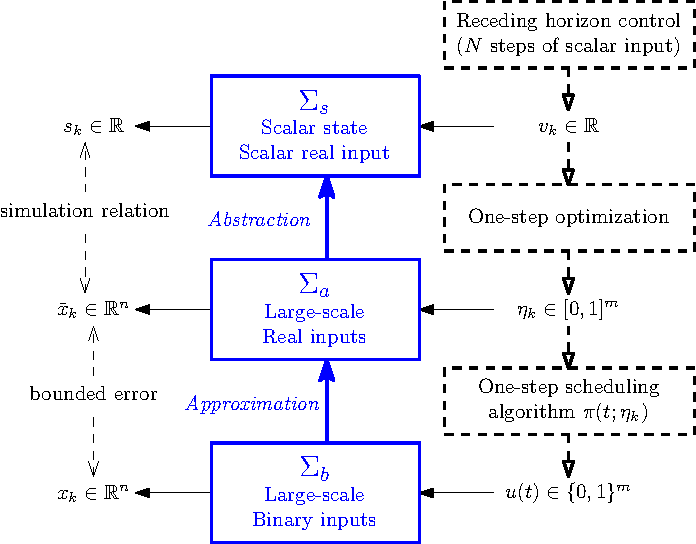
\includegraphics[width=\columnwidth]{approach_overview}
  \caption{Overview of the approach.}
  \label{fig:overview}
\end{figure}


%%% Local Variables:
%%% mode: latex
%%% TeX-master: "emsoft15gs"
%%% End:
